\section{Method}
\label{sec:method}

\subsection{Knowledge Resources}
\label{sec:resources}

\textit{AudioSet} \citep{gemmeke2017audio} is a hierarchically structured ontologies comprised of 632 audio events. It is by far the largest ontology, covering most common sound events. 
\textit{SONYC} \citep{bello2019sonyc} is a two-level taxonomy consists of 8 coarse level tags, 23 fine level tags about urban sounds. This taxonomy is smaller due to its specific target of detecting urban noises.
\textit{ASER} \citep{zhang2020aser} is a large-scale eventuality knowledge graph extracted from textual corpus. Each eventuality is represented as a short clause containing lemmatized words of subject, verb, object, etc. In this work, we will use its core version with 27,565,673 event nodes and 8,834,257 relation edges of 15 types. We will focus on temporal relations types like \textit{Precedence} and \textit{Conjunction}.
% In this work, we will use its core version with 27,565,673 event nodes and 8,834,257 relation edges, and focus on temporal relations like \textit{Precedence, Succession, Synchronous} and \textit{Conjunction}.

\subsection{Knowledge Construction}
\label{sec:enrich}
In this section, we will introduce how to perform the alignment between an audio event label set and ASER, and construct the temporal KG to enrich the existing ontologies (Figure \ref{fig:pipeline}) . Without loss of generality, we will mainly describe the procedure with AudioSet as target, and explain the difference for SONYC when necessary. 

\begin{figure}[htbp]
\setlength{\abovecaptionskip}{0.cm}
\setlength{\belowcaptionskip}{-0.5cm}
  \centering
  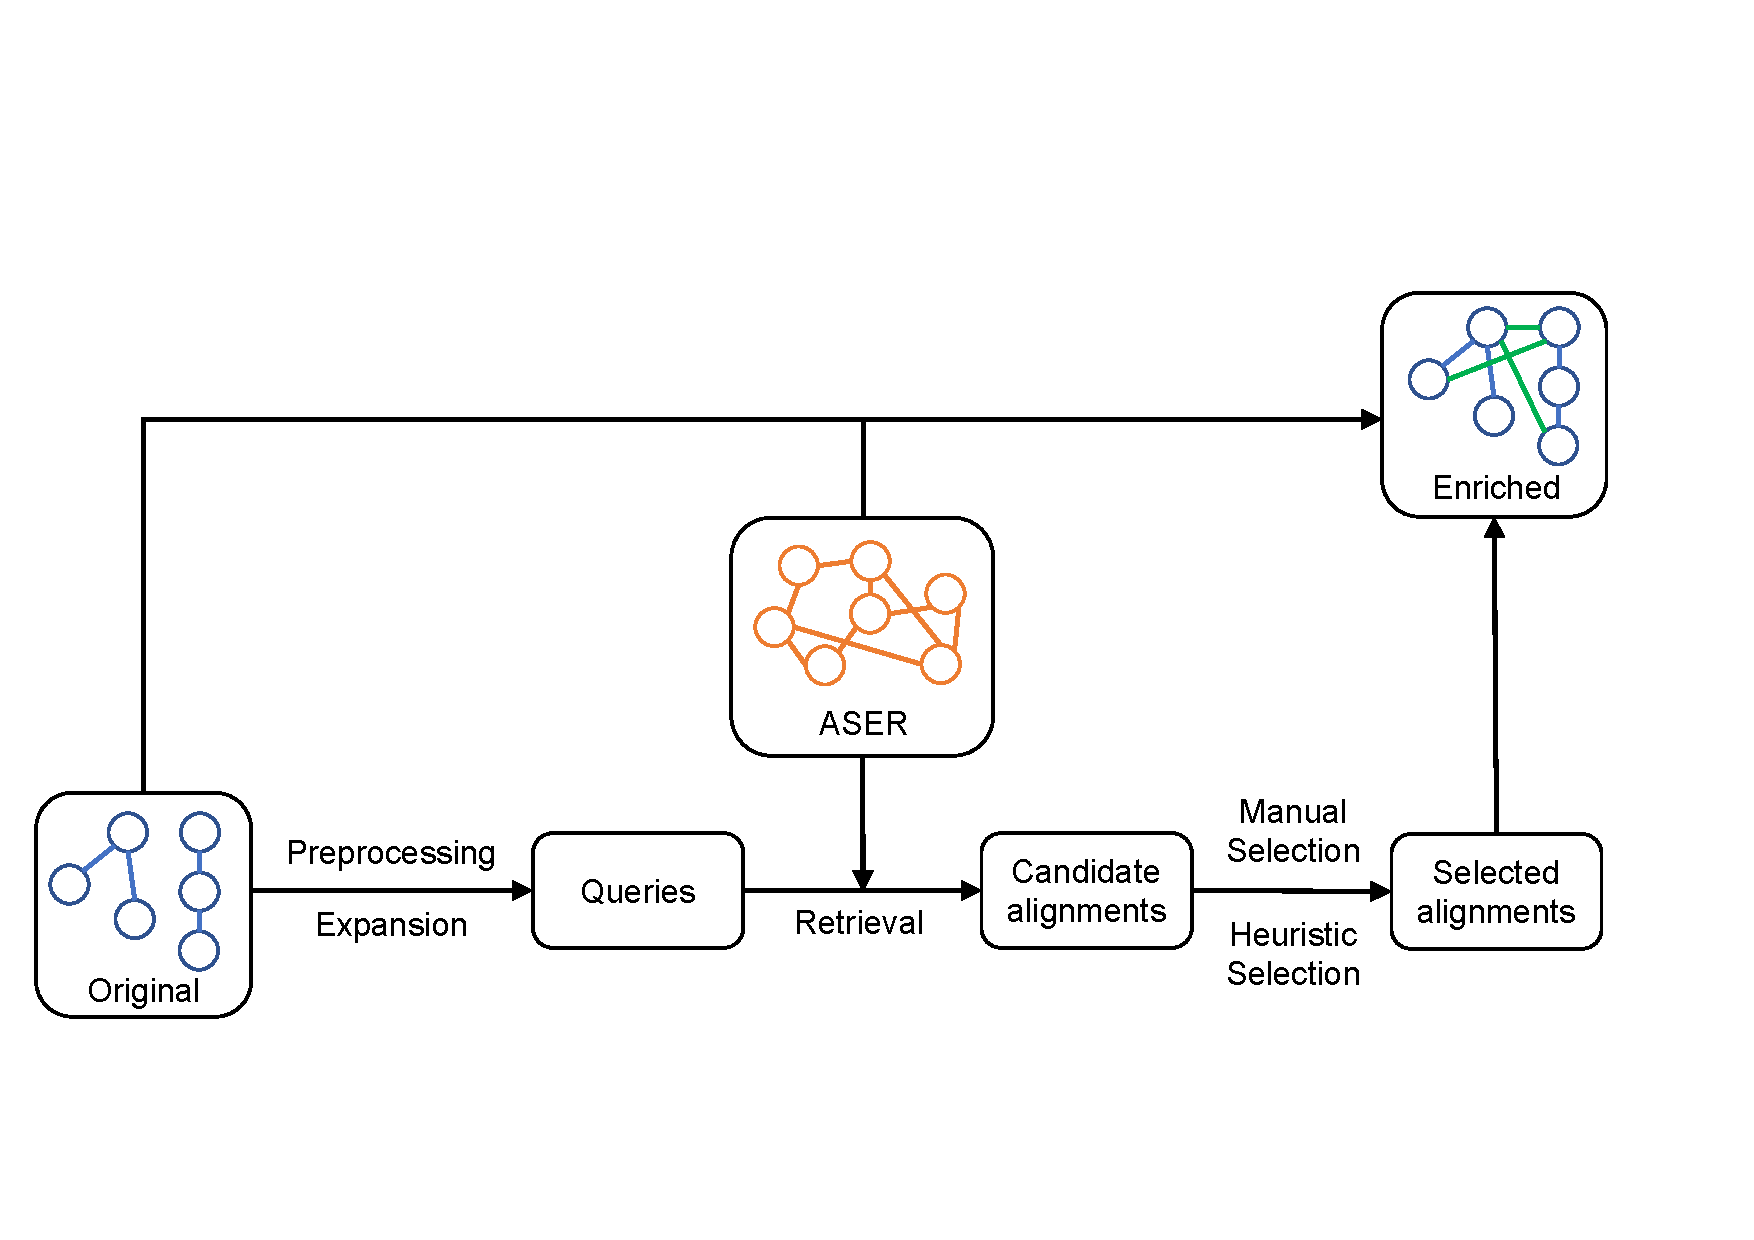
\includegraphics[width=1\linewidth]{figures/pipeline1.pdf}
  \caption{Illustration of alignment pipeline.}
  \label{fig:pipeline}
  \end{figure}

\subsubsection{Preprocessing and Expansion}

First, we conduct preprocessing to deal with the morphological differences between two type of representations. The words in ASER events are already lemmatized, while the verbs in AudioSet tags are not. Therefore, we enforce lemmatization on AudioSet tags, and also do lowercasing, remove the parentheses and stopwords. % for AudioSet tags. % remove "with spacy" detail

After that, since there are lexical variations in the expressions of similar audio events in ASER, we propose to expand a single AudioSet tag into multiple equivalent queries to improve the recall of alignment candidates retrieval (\S \ref{sec:cand-retrieval}). 

First, some of the tags already contain parallel concepts or synonyms, like ``Roaring cats (lions, tigers)'', and we will split it into multiple queries with one concept each, like ``roaring cats'', ``lions'' and ``tigers''. 
Moreover, for those tags without provided synonyms, we can also extract their synonyms from the lexical database WordNet \citep{miller1995wordnet}. To leverage the knowledge from WordNet, we applied the Lesk algorithm \citep{lesk1986automatic} for Word Sense Disambiguation (WSD) to link each word to its corresponding Wordnet synset. %with the implementation of pywsd \citep{pywsd14}. The event description provided in AudioSet can be utilized as the context to aid WSD along with the tag itself, while for SONYC, we apply WSD on the tag alone. 
There are also ambiguous events in AudioSet with multiple father events. For example, the event ``Hiss'' is a child event of ``Cat'', ``Snake'' and ``Steam'', and the acoustic property of the event might be different under different father events. Hence, we produce different queries by pairing such event with each of its father events, so the expanded queries for the above example would be ``cat hiss'', ``snake hiss'' and ``steam hiss''.

\subsubsection{Alignment Candidates Retrieval}
\label{sec:cand-retrieval}

Since ASER contains numerous events, we need to retrieve a small number of likely candidates before alignment selection. At first, we filter out some unlikely candidates by excluding events with noisy patterns like duplicate verbs (``I say say''), and infrequent ones (with frequency < 5). We then retrieve the top 10 events for each query with ElasticSearch. First, we adopt pure text-matching, and give higher weight to the matching of verbs, as verbs are the key components of events. Moreover, since we noticed that the above text matching approach may sometimes retrieve infrequent events that is either too rare or too specific, we also supplemented the above method with another weighting scheme that adds additional weights according to event frequency. Consequently, retrieval results will contain more general and frequent events, which will have more linked relations to leverage. The results from both weighting schemes are combined to balance accuracy and frequency. 
Finally, the retrieved ASER events with the multiple queries of the same AudioSet event are
aggregated as the candidates for alignment. As a result, each event has 31.3 candidates in average with a minimum of 2 and maximum of 190. 

\subsubsection{Selection} 

Now we need to select events that are precisely related to a sound event in terms of acoustic property from the retrieved candidates. 

For the alignments to AudioSet, we manually annotate them ourselves to ensure the reliability. We need to decide for each candidate eventuality of an AudioSet event, whether they are related, unrelated or that the relation is ambiguous. The event name, description, father/child events, corresponding queries and example videos containing that event are shown to aid the decision. Among all the annotated alignments, about 31.96\% are considered related, 13.52\% ambiguous and 54.51\% unrelated. To ensure the precision of the results, we only use the ``related'' alignments later.

For the alignments to SONYC, we completely automate the selection process. We observe that
most candidates for certain specific event labels (like ``Reverse Beeper'') are already of acceptable quality. Therefore, we preserve all the candidates of specific labels except ``other/unknown'' labels and under-specified labels like ``machinery impact''. % We will show in experiments that the resulting alignments are already beneficial for this task.

\subsubsection{Construction}

The relations between ASER events are transferred to their corresponding AudioSet events through the alignments, and their relations will be aggregated. For example, let's assume that an AudioSet event $a_1$ is aligned to events $e_{11}, e_{12}$, and another event $a_2$ is aligned to $e_{21}$. In ASER, $e_{11}$-$e_{21}$ has the relation \textit{(`Co\_Occurrence', `Conjunction')}, and $e_{12}$-$e_{21}$ has the relation \textit{(`Co\_Occurrence', `Precedence')}. Then $a_1$-$a_2$ will have the aggregated relation \textit{(`Co\_Occurrence', `Conjunction', `Precedence')}. The resulting KG will inherit various types of relations from ASER, and we will only use \textit{Conjunction} and \textit{Precedence} in later experiments as other relations are either not temporal or too sparse.
\subsection{Double GCN (D-GCN)}

Typically, CNN-based models \citep{kong2020panns} are used for audio tagging. To leverage KGs, we roughly follow \citep{wang2020modeling} to add a GCN component to learn the representation of labels. Then the audio representations from the CNN encoder are dot-producted with the learned label representations, followed by a sigmoid layer to get the prediction. 

Either the ontology or temporal KG alone can be incorporated into GCN-based models for audio tagging. However, a single GCN may not be suitable to handle the heterogeneity of two knowledge types when we want to combine their strength in one model. We thus draw inspiration from R-GCN \citep{schlichtkrull2018modeling}, which introduced relation-specific transformations.

\begin{equation}
\setlength{\abovedisplayskip}{3pt}
\setlength{\belowdisplayskip}{3pt}
  h_i^{l+1} = \sigma(\sum_{r \in \mathcal{R}} \sum_{j \in N^r_i} \frac{1}{c_{ij, r}} W^{l}_r h^{l}_j)
\end{equation}
where $h_i^{l}$ are the features of node $i$ at the $l$-th layer, $\mathcal{R}$ is the set of relations, $N^r_i$ is the indices of the neighbors of $i$ via edges with relation $r$ (self-loop included), $c_{ij, r}$ is a normalization constant, and $W^{l}_r$ is the specific weight matrix for relation $r$ at the $l$-th layer. The original R-GCN also introduce basis function decomposition and block decomposition for $W^{l}_r$ as a regularization to reduce parameters and prevent overfitting on rare relations.

Different from the original R-GCN, which aims to tackle the completion of knowledge bases with over 1,000 relation types, we only need to model 2 kinds of relations with relatively balanced numbers. Therefore, we don't apply the regularizations and further add relation specific bias terms, to improve the model's expressiveness on each relation. We will refer to this variant as D-GCN.
